
%%%%%%%%%%%%%%%%
%%% ANALYSIS %%%
%%%%%%%%%%%%%%%%

\chapter{Analysis}

% Design principles, inspiration, methodology

The thesis investigated here is that using tabletops as basic Input/Output peripherals for other computing devices will help their adoption by the masses.
A user should be able to transfer the display of his/her device to a tabletop, and interact with it without any further complications.
To demonstrate the feasibility of this interaction model, an analysis of the requirements is conducted, leading to the design and implementation of a prototype application.
\\\\
The application UI consists of two elements.
\begin{itemize}
\item{The \emph{virtual screen} provides the user with a clone of his/her device's display, and forwards touch input to the same device. As such, it is device specific and requires no interface design.}
\item{The \emph{application interface} provides the user with ways to manipulate the virtual screen. It needs to be designed and implemented on the tabletop.}
\end{itemize}





\section{Context of use}

\subsection{Scenarios}

\subsubsection{The coffee shop}

\begin{quotation}
\small{
Alice is in a Coffee Shop, waiting for her friend Bob. She is sitting at an interactive table, which allows her to order her drink via a digital interface, as well as supports TableShare technology.

She takes her phone and notebook out of her purse and places them on the table. A dialog pops up on her smartphone, asking her to confirm the UI transfer, which Alice does by a simple touch. A simple menu appears on the table beside her phone. Alice taps the �Expand� tab, and her phone�s screen appears on the table beside her phone, as a same size mirrored display.

She resizes the window to her convenience, and moves it closer to her by sliding her phone on the surface. The screen goes gray to notify Alice that an object (the notebook) is in the way. Alice removes the notebook, and the window becomes active again. She accesses her phone�s applications, and starts typing an email.

When Bob arrives, Alice minimizes her display, keeping her phone in place. Bob orders a drink and they start catching up. After a while, Bob leaves. Alice restores her phone�s screen, finishes up her email, and disconnects TableShare by simply lifting the phone off the table.}
\end{quotation}

\subsubsection{The meeting}

\begin{quotation}
\small{
Jim, Jack and Jill are having a meeting about the development of a product. They are sitting around an interactive table, with different artefacts, including paper, pens, computing devices and coffee cups. Jill is responsible for the meeting�s agenda, which is stored on her smartphone.

Jill places her phone on the top right corner of the table and establishes a UI transfer via TableShare. She uses the �Grab� tap to drag the display window to the left of the phone where there is space. She opens the document containing the agenda, and uses the �Resize� corner of the window to enlarge the display, so as to allow convenient visual reference for all present.

It is now time for Jack to present a diagram of the development process. He switches on his tablet computer, opens said diagram, and places the tablet on the table for the others to see. The screen is however too small, so Jack decides instead to use the TableShare application. With a single tap on the �Grab� tab, Jack pins the UI to the table, allowing him to remove the physical tablet while keeping the mirrored display active. By using the �Resize� corner, he enlarges and flips the orientation of the window to a landscape display. By the use of a double touch on the �Grab� tab and the active window, Jack rotates the display to a convenient position, and presents the diagram to his colleagues. When done, Jack minimize the window by tapping the �Retract� tab. The window takes the shape of an active icon, ready to be restored or closed as convenient. When the meeting is over, Jack taps the �Close� tab on the icon to interrupt TableShare.}
\end{quotation}

\subsubsection{The office}

\begin{quotation}
\small{
It is monday morning and Bill arrives at his office. His working desk is made up of an interactive table, extended with a vertical screen, mouse and keyboard. On it are various physical objects, including a stack of papers, some books, pens, an empty cup and a lamp.

Bill wakes the tabletop up from its standby state by simply placing his smartphone on it. The devices know each other, so TableShare is automatically launched. Bill uses the TablePush widget on his phone to push other widgets to the table space. Bill places his calendar up in one corner, together with his Skype widget.

After reading through his mail on the vertical screen, Bill starts typing an answer using the keyboard. He needs to refer to a document that is stored on his phone. Bill and uses the �Grab� tab beside his phone to attach its display beside the device. He enlarges the window and moves the display to a convenient location by sliding the phone. Bill types on..

Suddenly the phone rings. Bill taps the �Grab� tab to effectively pin all applications and UI display to the tabletop, allowing him to pick up the phone without interrupting the UI transfer.}
\end{quotation}

\subsection{Storyboards}

Interest of storyboards

\section{Application requirements}

\subsection{Hardware constraints}

\subsubsection{Design concerns for tabletops}

A tabletop computer is ..

.. a situated device:

not mobile

public

interruptions in interaction flow

.. a table:

horizontal working surface

concurrent activities on table: other apps, other devices (papers, cup..)

limited (screen) space availability

reach issue

.. an interactive surface:

use of Tangible UIs possible

input techniques: fingers (gestures), pen, mouse, other devices

use of screen space: drag/resize/rotate, touch areas, full screen

.. a shared device:

user identification/authentication (virtual lenses, NAI
privacy/security

multi-user scenarios: collaborative/parallel

.. a computer:

specs, platform, hardware ??

network capabilities

\subsubsection{Designing for mobile devices}

\subsection{Software components}

\subsubsection{Detection and discovery}

\subsubsection{Display transfer}

\subsubsection{Surface user interface}

\subsection{Choice of features}

\section{Interaction design}

\subsection{Generating ideas with low fidelity prototypes}

%\begin{figure}[h!]
%  \caption{Low fidelity prototypes.}
%  \centering
%    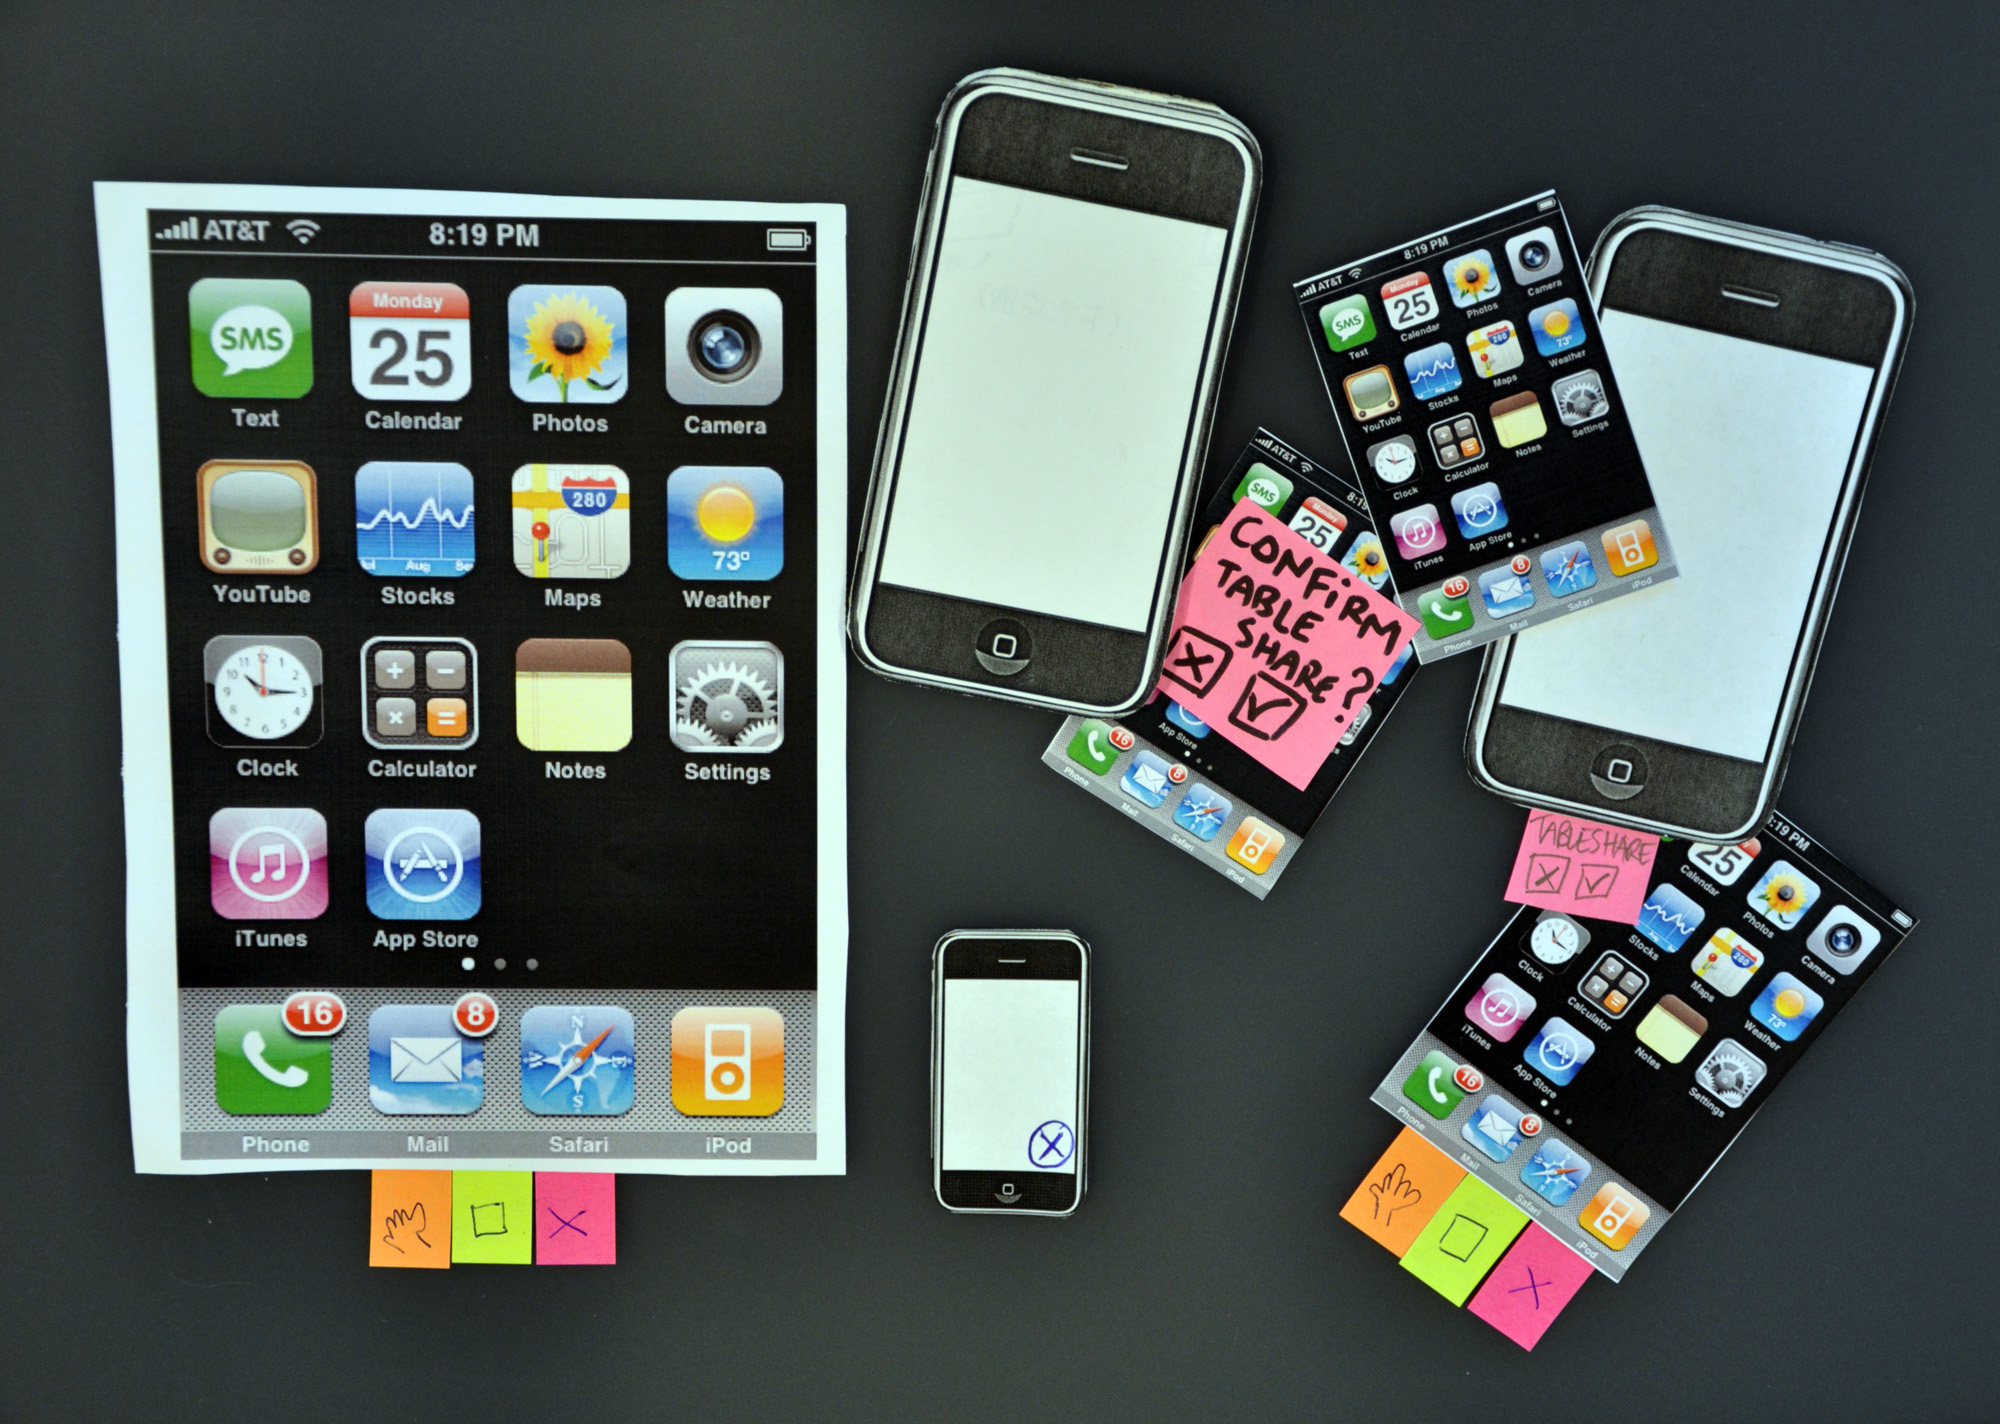
\includegraphics[width=0.8\textwidth]{images/paperprot1}
%\end{figure}
%
%\begin{figure}[h!]
%  \caption{Low fidelity prototypes.}
%  \centering
%    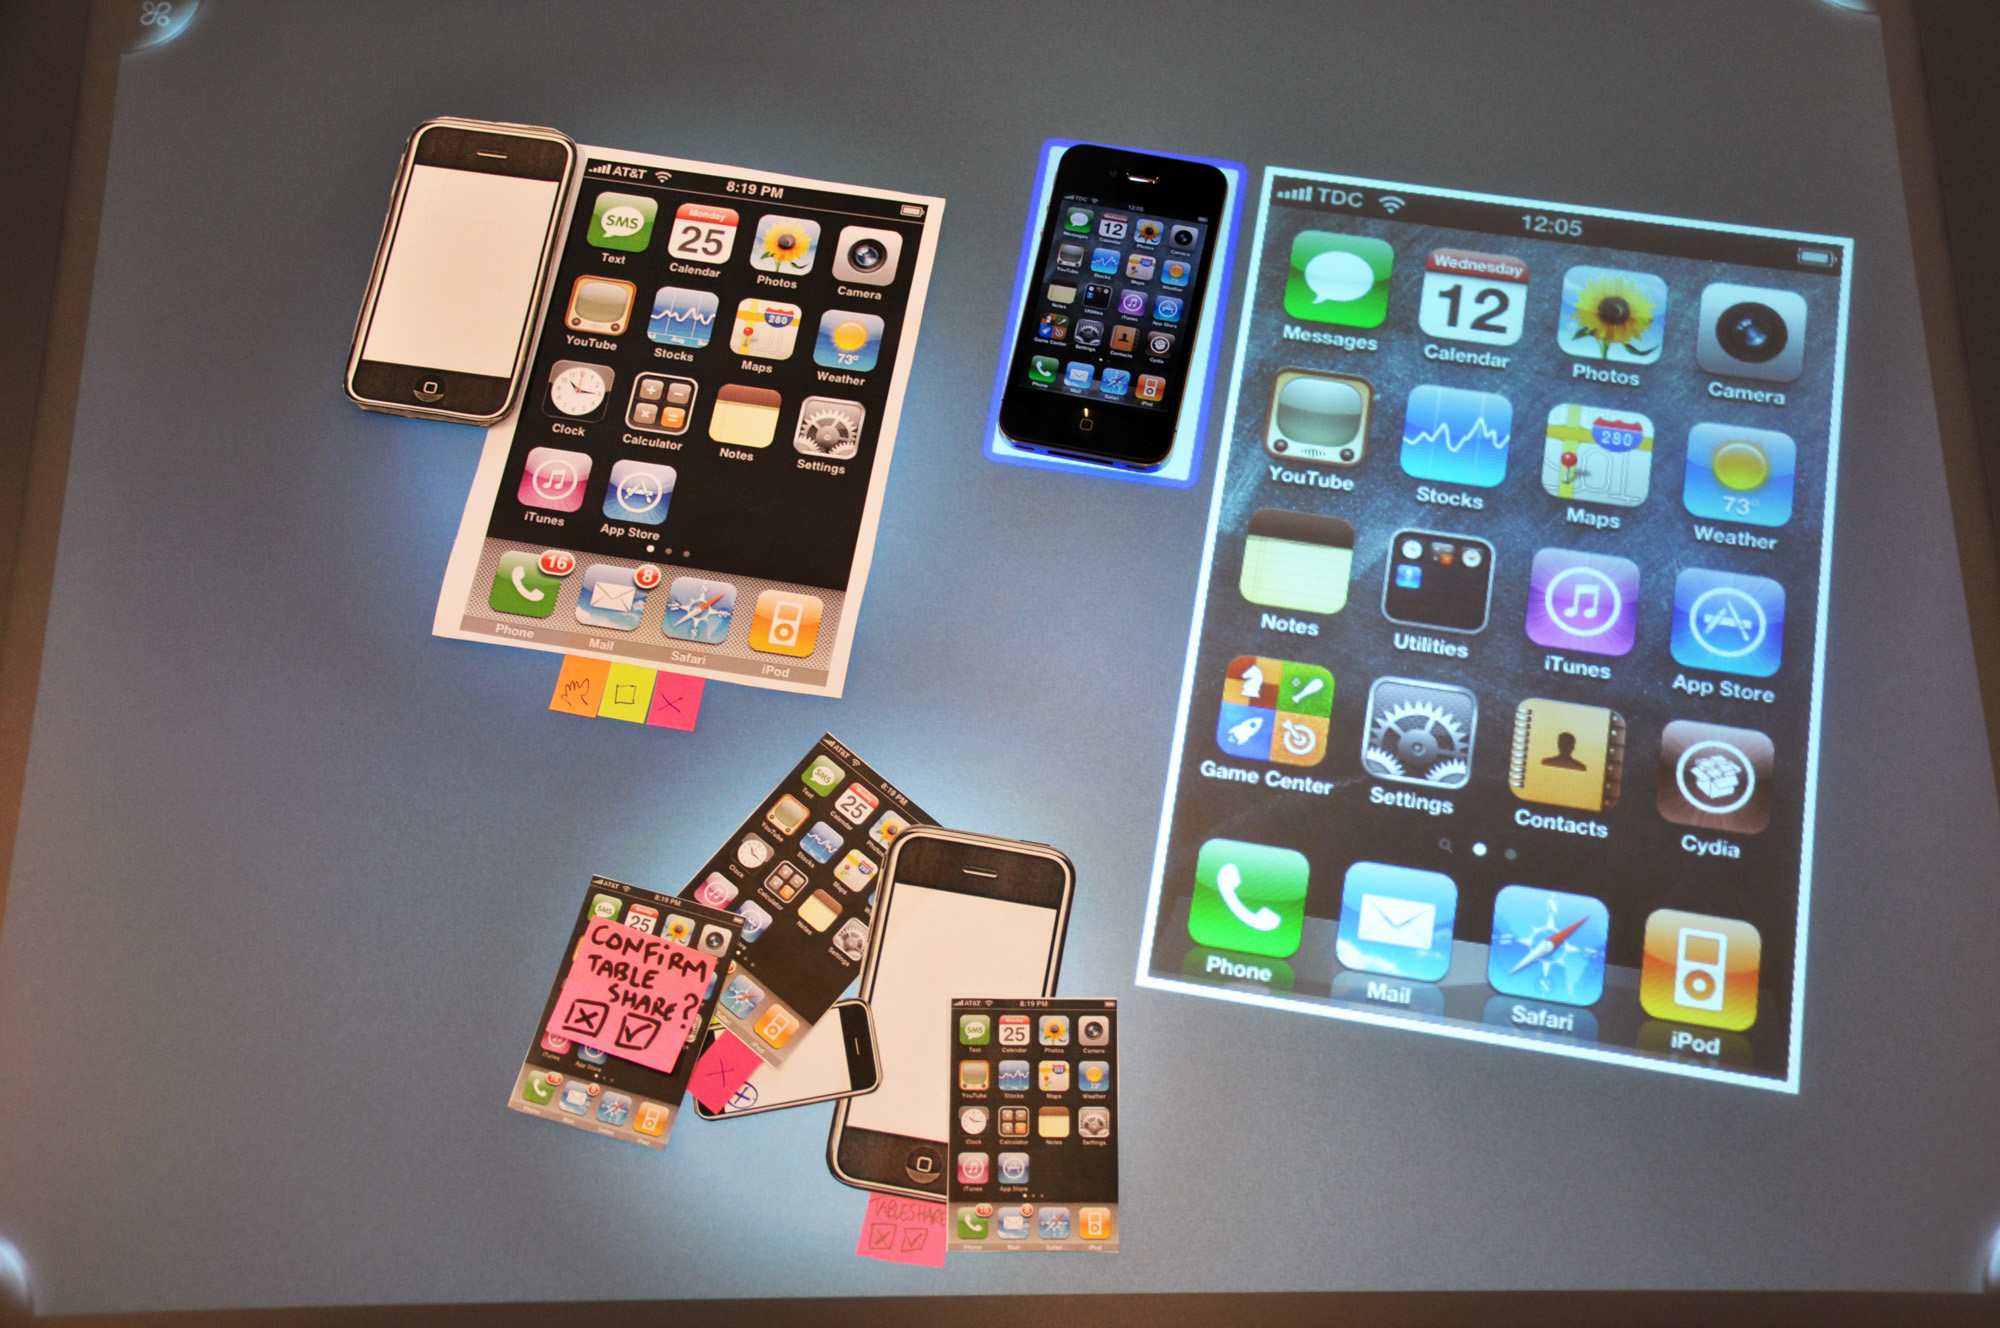
\includegraphics[width=0.8\textwidth]{images/paperprot2}
%\end{figure}
%
%\begin{figure}[h!]
%  \caption{Low fidelity prototypes.}
%  \centering
%    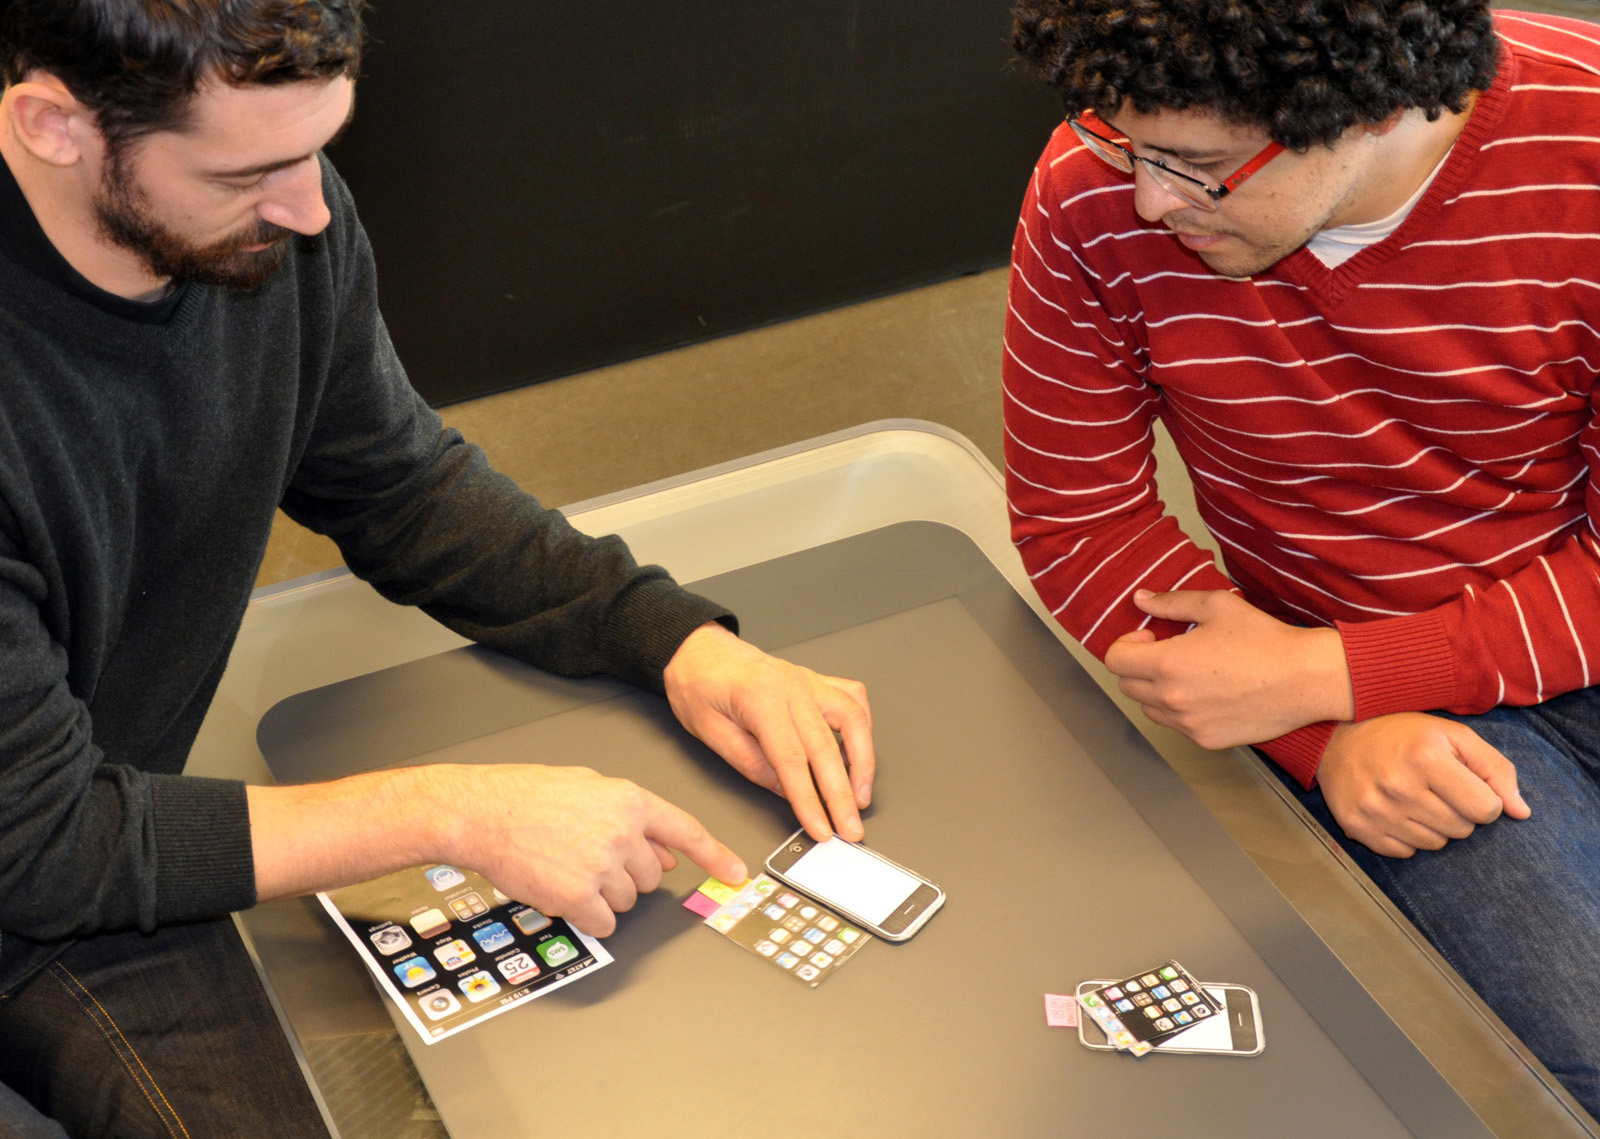
\includegraphics[width=0.8\textwidth]{images/paperprot3}
%\end{figure}

\subsection{Commands and actions}

Human computer interaction can be modeled as a simple cause-effect relationship.

The user wishes the computer to execute a command.
To achieve that, he/she performs an action, making use of the available input devices (keyboard, mouse, etc..) and interfaces.
The action is the cause, the command is the effect, and together they form a single interaction between user and machine.

On an interactive surface, the traditional input devices are gone, and the interaction is based on hand gestures.

Those concepts are inspired by the paper ``User-Defined Gestures for Surface Computing'' by Wobbrock, \cite{Wobbrock:2009:gestures}.

The following six basic commands (interaction primitives) were identified and progressively chosen as being essential to the TableIO application.

\begin{enumerate}
\item{\emph{Dragging} the application window across the interactive surface.}
\item{\emph{Rotating} the application window across the interactive surface.}
\item{\emph{Resizing} the application window across the interactive surface.}
\item{\emph{Minimizing} the application window, making it possible to restore it easily.}
\item{\emph{Hiding} the content of the application window.}
\item{\emph{Exiting} the application, thus closing the application window.}
\end{enumerate}

EXTRA command: device buttons (HOME on the iPhone) should be supported.

\subsection{Interaction strategies}

Various interaction techniques can be used to invoke application level commands.

Early idea generation process lead to the definition of  specific interaction strategies.

Each strategy can be consistently implemented for each previously defined command.

\begin{enumerate}
\item{\emph{Action Tabs} are traditional buttons/tabs that implement functionalities.}
\item{The \emph{Action Bar} can be compared to a virtual touchpad, it includes a manipulation area and buttons.}
\item{\emph{Window Toggle} refers to using a switch to toggle the window between inactive and active states. In its inactive state, the window is made manipulable as a common digital picture.}
\item{The \emph{Active Border} is a digital frame around the application window used for manipulation.}
\item{\emph{Active Corners} is a strategy similar to Active Border, with the difference that the border's corners implement specific functionalities.}
\item{\emph{Other} regroups suggestions that do not fit with any specific strategy.}
\end{enumerate}

\section{Preliminary usability study}

A well-designed product is a successful one.
Usability and appeal are key elements towards the success of an application.
The goal of this experiment is to gather knowledge directly from users to inform important design decisions.

Example of designers designs that fails from user standpoint.

The goal is to have potential users of the system describe their ideal user interface.

The focus of the experiment is not the interaction with the mirrored smartphone's screen.
The focus is the manipulation of the application window that contains the mirrored display.

\subsection{Method}

\subsubsection{Parameters}

The parameters of the experiment are the above mentioned commands and actions.
The 6 commands form a set of features that are considered necessary for the application to function.

For each of the chosen commands, we have 6 implementation suggestions (1 for each interaction strategy).

\subsubsection{Participants}


\subsubsection{Experiment}

The experiment is based on low fidelity prototypes.
Instead of a digital user interface, the participant interacts with paper representations.

The user is asked to perform a task using the application.
The task is divided into the 6 actions that 


\subsection{Results}



Comments:
users suggest dragging/rotating the window directly (forget that window forwards input to device)

LIMITS:
UNFORTUNATELY, results are biased due to splitting the suggestions in 2, for each participant group.
Ranking result for 1 strategy is only valid compared to 2 other suggestions from same participant group, not valid across all strategies.